\documentclass[12pt,a4paper]{article}
\usepackage[T1]{fontenc}
\usepackage[utf8]{inputenc}
\usepackage[italian]{babel}
\usepackage{lmodern}
\usepackage{graphicx}
\usepackage{minted}
\usepackage{hyperref}
\usepackage{dirtree}

\setlength{\parindent}{2em}
\setlength{\parskip}{1em}

\setlength{\abovecaptionskip}{.8em plus .3em minus .3em}
\setlength{\belowcaptionskip}{.8em plus .3em minus .3em}

\setminted{encoding=utf-8,outencoding=utf-8,frame=lines,framesep=1em}
\renewcommand{\listingscaption}{Listato}

\newcommand{\mrcnn}{Mask-R\_CNN}

\title{Riconoscimento Documenti}
\author{Simone Cimarelli \and Vittorio Mignini \and Luca Moroni}
\date{9 luglio 2020}

\begin{document}

\maketitle

\begin{abstract}
    Si descrive l'implementazione di un applicativo che permette il
    riconoscimento in tempo reale di un set estensibile di tipologie di
    documenti.
\end{abstract}

\section{Obbiettivi}

Implementare un applicativo che tramite l'utilizzo di un dispositivo di
input video sia in grado di riconoscere e di identificare un insieme
estensibile di documenti e di riconoscere delle porzioni di testo
presenti in essi.

\section{Analisi dei Requisiti}
\subsection{Analisi dei Requisiti Utente}

\begin{itemize}
    \item Ottenere un elenco dei documenti visibili all'interno di
        un'immagine e le componenti testuali specifiche in essi
        riconoscibili.
    \item Avere la possibilità di definire la natura dei documenti
        oggetto del riconoscimento e delle informazioni testuali
        rilevanti in essi contenute.
    \item Mettere a disposizione un'interfaccia grafica semplice e
        minimale per l'acquisizione di video e immagini.
    \item Implementare delle tecnologie per l'object detection e ocr
        allo stato dell'arte per erogare in modo efficiente il servizio
        richiesto dal committente.
\end{itemize}

\subsection{Glossario e Dominio applicativo}

Il prodotto risponde all'esigenza di individuare la tipologia ed
eseguire il riconoscimento dei prinicipali dati testuali esposti in vari
documenti identificativi tramite webcam. I domini applicativi di tale
sistema e le problematiche ad essi connesse sono sono quelli dell'ambito
della computer vision e dell'OCR. L'utente finale avrà a disposizione
un'interfaccia grafica attraverso la quale, in modo intuitivo ed
efficiente, potrà avere accesso al servizio erogato.

\begin{description}
    \item[Computer Vision] Insieme di metodologie algoritmiche e
        matematiche che hanno come obiettivo quello di acquisire delle
        conoscenze ad alto livello partendo da immagini o video. Nel
        nostro caso capire se e dove nello stream video esaminato
        dall'applicativo è presente un documento di uno dei tipi
        prestabiliti.
    \item[Object Detection] Tecnologia relativa all'ambito della
        computer vision che propone una soluzione algoritmica per il
        riconoscimento di istanze di oggetti appartenenti a classi
        predefinite in immagini digitali e video.
    \item[OCR] Optical Character Recognition, metodologie software per
        il riconoscimento di caratteri contenuti in immagini traduzione
        di tali simboli in caratteri digitali equivalenti.
\end{description}

\subsection{Modellazione Concettuale del Sistema}

La logica del sistema sarà divisa in due macro blocchi: il compito di
interagire con l'utente finale sarà a carico di una componente di
interfaccia grafica ``frontend'' che si occuperà di interfacciarsi alla
videocamera e di mostrare uno storico dei documenti riconosciuti e in
corso di riconoscimento in tempo reale; il compito di applicare e
interpretare i risultati delle primitive di riconoscimento e OCR sarà
invece delegato a una componente ``business logic''. Il committente
avrà la possibilità di configurare questa componente scegliendo il tipo
di documenti da riconoscere e le caratteristiche testuali da ricercare.

\subsection{Diagramma di caso d'uso}

In fase di revisione dei requisiti, siamo andati a definire con maggior
precisione i requisiti funzionali del nostro applicativo tramite
l'utilizzo del diagramma di caso d'uso.

Tale diagramma, necessario nella prima fase di progettazione, ha
permesso di definire quella che è a grandi linee la logica di
funzionamento del nostro
sistema per quanto riguarda i casi d'uso ``riconoscimento'' e ``configurazione''.

\begin{figure}[H]
    \caption{Diagramma di Caso d'Uso}
    \centering
    \includegraphics[width=\textwidth,height=\textheight,keepaspectratio]{uml_use_case.pdf}
\end{figure}

\subsection{Specifica di caso d'uso ``riconoscimento''}
\begin{description}
    \item[Attori:] utente
    \item[Precondizioni:] l'utente ha posizionato a favore di camera un
        documento
    \item[Sequenza degli eventi:] il sistema processa lo stream video
        tramite primitive di object detection e OCR estrapolando i
        documenti in esso contenuti con i relativi dati testuali.
    \item[Postcondizioni:] l'utente avrà a disposizione i risultati
\end{description}

\subsection{Specifica di caso d'uso ``configurazione''}
\begin{description}
    \item[Attori:] admin
    \item[Sequenza degli eventi:] il sistema mette a disposizione
        dell'admin strumenti per l'aggiunta di nuove tipologie di
        documenti e per la modifica di eventuali impostazioni dello
        stesso
    \item[Postcondizioni:] le modifiche apportate al sistema e alle
        tipologie di documenti saranno confermate.
\end{description}

\section{Architettura del Sistema}

\subsection{Scelte architetturali}

Nella progettazione architetturale dell'applicativo, abbiamo utilizzato
librerie testate e rappresentanti lo stato dell'arte del dominio
applicativo. Per quanto riguarda l'object detection, abbiamo selezionato
\textbf{\mrcnn}, una libreria che oltre a effettuare object detection
per mezzo di una rete neurale convoluzionale, mette a disposizione anche
la segmentazione di immagini, una feature aggiuntiva che oltre a
ritornare i rettangoli contenenti gli oggetti di una determinata classe
presenti nell'immagine ne ritorna anche la regione di pixel che li
rappresenta. Tale feature non sarà utilizzata nel nostro sistema, ma si
dimostra utile in fase di training
(v.~§\ref{s:training}~\nameref{s:training}) in quanto rende possibile
specificare l'area dei documenti contenuti nelle immagini di training in
maniera molto precisa, evitando ad esempio la l'inclusione dei
polpastrelli che in alcuni casi possono influenzare il comportamento
della rete. Per effettuare l'OCR abbiamo optato per la libreria
tesseract, resa disponibile in python tramite il modulo wrapper
pytesseract. Le librerie appena citate hanno determinato la necessità di
importarne altre tra cui tensorflow$=$1.x e keras$=$2.0.8 sulle quali si
basa \mrcnn, ed OpenCV2 per la gestione e la codifica delle immagini.

Per la gestione delle dipendenze abbiamo utilizzato due strumenti propri
dell'ambiente python. \texttt{pipenv} crea un ambiente virtuale
contenente le specifiche versioni delle librerie utilizzate separando
queste rispetto a quelle di sistema e rende ripetibile su altre macchine
l'esatta configurazione da noi utilizzata. \texttt{pyenv} permette di
utilizzare una versione specifica dell'interprete python diversa da
quella fornita dal sistema. Nel nostro caso, tensorflow$=$1.x è
compatibile solamente con versioni di python$\leq$3.7.x con
\texttt{pyenv} tale requisito può essere soddisfatto su qualsiasi
macchina.

Data la complessità computazionale delle operazioni impiegate
dalle librerie \mrcnn\ e tesseract, si è optato per effettuare
l'elaborazione di singoli frame, e non di uno stream video
continuo, questo perché non sarebbe garantita una buona fluidità
del servizio a meno di impiegare una macchina server estremamente
performante, e quindi costosa.

\subsection{Accenni strutturali su \mrcnn}

La logica della rete \mrcnn\ prevede l'esecuzione di due fasi. Nella
prima fase la rete ritorna delle regioni che dovrebbero rappresentare
oggetti presenti all'interno dell'immagine di input. La seconda fase
invece effettua un inferenza sulle classe degli oggetti, rifinisce le
bounding box (ROIs, regioni di interesse) e genera le maschere a livello
di pixel basandosi sull'output della prima fase. Entrambe le fasi sono
connesse alla struttura backbone.

\begin{figure}[H]
    \caption{Struttura di \mrcnn}
    \centering
    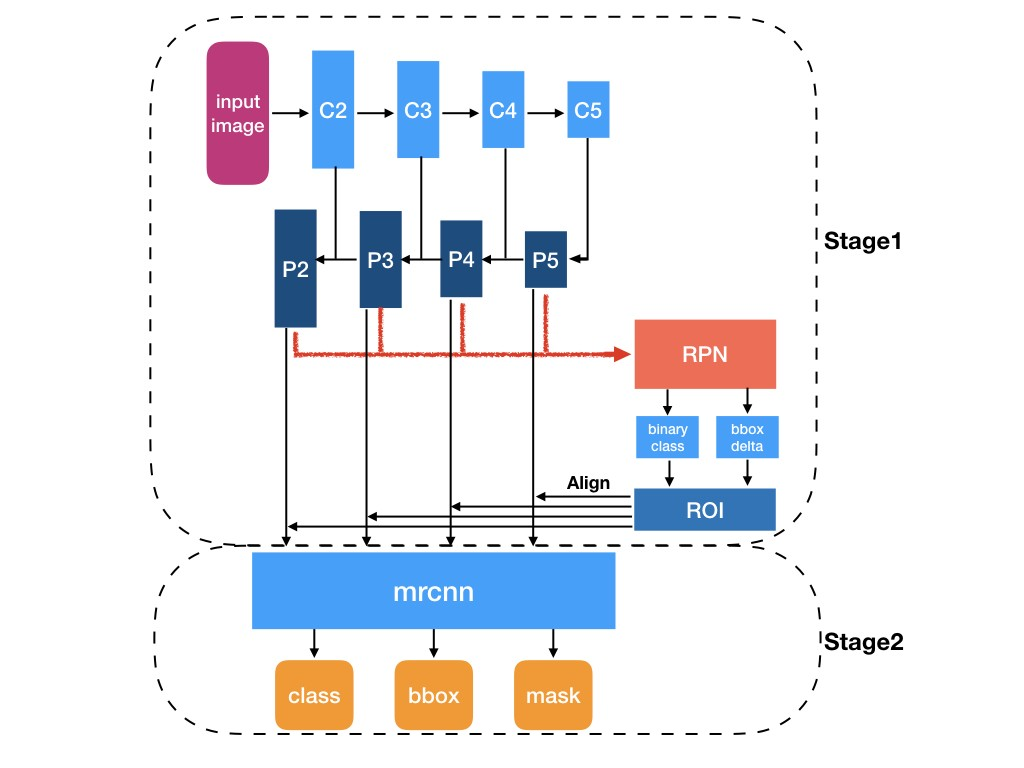
\includegraphics[width=.88\textwidth]{mask_description.jpg}
\end{figure}

\subsection{Training}
\label{s:training}

Per training di una rete neurale intendiamo la sequenza di operazioni
eseguite al fine di modulare i valori interni (pesi) che influenzano il
comportamento dei nodi della rete, con il fine ultimo di abbassare il
tasso di errore associato alle previsioni della rete.

La bussiness logic del nostro sistema si basa su una rete neurale per la
computer vision implementata dalla libreria \mrcnn\ sulla quale facciamo
\textit{transfer learning}, ovvero eseguiamo training solo sugli strati
più esterni adattando la struttura della rete al riconoscimento di un
certo numero di classi di oggetti definibili dall'amministratore,
prendendo i pesi per gli strati inferiori dal modello MS COCO.

Per eseguire il training della rete ci siamo appoggiati alla potenza
computazionale fornita gratuitamente da Google tramite il servizio Colab
Per rendere ripetibile queste operazioni sulla base delle future
necessità del committente abbiamo reso disponibile il dataset e il
notebook Jupyter da noi utilizzati, così da avere una base su cui
espandere per il tuning dei parametri di training, l'aggiunta di nuove
classi di documenti e l'ampliamento del dataset. Una copia per la
consultazione del notebook in questione è visionabile alla fine di
questo documento.

Si rimanda infine all'applicativo web utilizzato per la
creazione di annotazioni per le immagini incluse nel dataset:\\
\url{http://www.robots.ox.ac.uk/~vgg/software/via/}

\subsubsection{Dataset}

La cartella del dataset contiene tre sottocartelle: training, validating
e testing. Le cartelle training e validating sono a loro volta divise in
ulteriori sottocartelle, una per ogni tipo di documento. Queste
sottocartelle contengono le foto da utilizzare nelle rispettive fasi di
allenamento della rete neurale e i metadati ad esse associati contenuti
in un unico file \texttt{via\_regions.json} presente in ogni
sottocartella. I nomi di queste sottocartelle non sono particolarmente
importanti, ma si consiglia di sceglierli in modo che siano descrittivi
delle immagini in esse contenute. In effetti, non è strettamente
necessario creare una nuova sottocartella ogni volta che si vuole
aggiungere una nuova classe di documento: anche la classe del documento
contenuto in una foto è infatti specificata nel file
\texttt{via\_regions.json}; la stessa sottocartella può quindi contenere
immagini che si riferiscono a classi di documenti diverse senza alcun
problema.\\ La cartella testing contiene invece foto da utilizzare
quando si volesse eseguire un test manuale dei risultati del training in
Colab.

\begin{figure}[H]
    \caption{Esempio di struttura di una cartella dataset}
    \centering
    \fbox{%
        \begin{minipage}{\textwidth}
            \dirtree{%
                .1 dataset.
                    .2 training.
                        .3 tesserino.
                            .4 tesserino1.jpg.
                            .4 ....
                            .4 tesserinoN.jpg.
                            .4 via\_regions.json.
                        .3 patente.
                            .4 patente1.jpg.
                            .4 ....
                            .4 patenteN.jpg.
                            .4 via\_regions.json.
                    .2 validating.
                        .3 tesserino.
                            .4 tesserino1.jpg.
                            .4 ....
                            .4 tesserinoN.jpg.
                            .4 via\_regions.json.
                        .3 patente.
                            .4 patente1.jpg.
                            .4 ....
                            .4 patenteN.jpg.
                            .4 via\_regions.json.
                    .2 testing.
                        .3 test0.jpg.
                        .3 ....
                        .3 testN.jpg.
            }
        \end{minipage}
    }
\end{figure}

Di seguito è riportato il contenuto di un file
\texttt{via\_regions.json} a titolo esemplificativo.

\begin{listing}[H]
    \caption{Esempio di file \texttt{via\_regions.json}}
    \inputminted{json}{via_regions.json}
\end{listing}

\subsection{Architettura di implementazione}

Abbiamo optato per lo sviluppo di una soluzione basata su tecnologie
web; andremo quindi a descrivere la progettazione di una web
application. Il nostro sistema sarà suddiviso in tre macro-parti:

\begin{itemize}
    \item Il \textit{frontend}, implementato tramite tecnologie web
        JavaScript, HTML e CSS
    \item Il \textit{backend}, realizzato in python tramite il
        framework flask per l'implementazione di servizi web.
    \item Il modulo di \textit{core business}, ovvero il nucleo
        dell'applicativo, sviluppato in python, per i compiti di object
        detection e di OCR
\end{itemize}

Nel seguito si andranno a descrivere i diagrammi UML utilizzati in fase
di progettazione e analisi architetturale nello sviluppo del nostro
sistema.

\subsubsection{Diagramma di classe completo}

Si descrivono le classi presenti nella logica del nostro applicativo.
Per lo sviluppo del frontend e del backend non è stata necessaria la
concettualizzazione di alcuna classe, causa approccio imperativo delle
tecnologie utilizzate.

In tale diagramma possiamo evidenziare tre package: \texttt{mrcnn}
rappresenta le classi della libreria \mrcnn, con cui i nostri moduli
andranno a utilizzare, descritte con un livello di dettaglio
semplificato e adeguato alle nostre esigenze. \texttt{training}
rappresenta le classi utilizzate durante il training della rete
(v.~§\ref{s:notebook}~\nameref{s:notebook}). \texttt{documentCNN} si
riferisce al modulo di core business da noi sviluppato.

\begin{figure}[H]
    \caption{Diagramma delle Classi}
    \centering
    \includegraphics[width=\textwidth,height=\textheight,keepaspectratio]{uml_class.pdf}
\end{figure}

\subsubsection{Diagramma di stato per l'oggetto Detectron}

Si descrive il diagramma di stato dell'oggetto Detectron proprio del
modulo di core business durante il suo ciclo di vita  nel nostro
applicativo.

Vengono individuati quattro stati nel quale l'oggetto trovarsi: lo stato
\textit{Created} che indica che il nostro oggetto contiene un modello di
\mrcnn\ ma non ha ancora i pesi caricati e quindi non può effettuare
alcuna inferenza, lo stato \textit{ReadyForInference}, indica che il
modello contenuto ha i pesi generati dalla fase di training caricati ed
è pronto per effettuare inferenza, lo stato \textit{Recognizing}, indica
che il nostro oggetto Detectron ha decodificato l'immagine e sta
aspettando il ritorno dell'inferenza dal modello della libreria \mrcnn.

Una volta disponibili i risultati dell'inferenza, se non sono state
trovate delle regioni di interesse che rappresentano documenti
nell'immagine, allora si ritorna nello stato di
\textit{ReadyForInference}; nel caso contrario passerà nello stato di
\textit{OCR Operations} nel quale il nostro oggetto effettuerà OCR sulle
ROIs tramite le funzioni esposte da pytesseract. Finite tali operazioni
ritornerà nello stato di \textit{ReadyForInference}.

\begin{figure}[H]
    \caption{Diagramma di Stato}
    \centering
    \includegraphics[width=\textwidth,height=\textheight,keepaspectratio]{uml_state.pdf}
\end{figure}

\subsubsection{Diagrammi di sequenza e comunicazione per il caso d'uso ``riconoscimento''}

Si descrive la logica del funzionamento del caso d'uso riconoscimento
tramite i diagrammi di sequenza e comunicazione. Come rappresentato il
nostro sistema mette in gioco varie componenti: il nostro attore
principale si interfaccia con una componente ``frontend'', che eseguirà
un loop nel quale andrà a prelevare un frame dall'input video,
inviandolo quindi alla componente ``backend'', implementata nell'oggetto
\texttt{app}, che passerà l'immagine all'oggetto di core business di
classe \texttt{Detectron}, il quale tramite l'utilizzo di metodi e
primitive proprie delle librerie \mrcnn\ e pytesseract creerà un
dizionario contenente per ogni documento i dati riconosciuti.

\begin{figure}[H]
    \caption{Diagramma di Sequenza}
    \centering
    \includegraphics[width=\textwidth,height=\textheight,keepaspectratio]{uml_seq.pdf}
\end{figure}

\begin{figure}[H]
    \caption{Diagramma di Comunicazione}
    \centering
    \includegraphics[width=\textwidth,height=\textheight,keepaspectratio]{uml_comm.pdf}
\end{figure}

\subsubsection{Diagramma di attività per la cattura e il processing di un frame}

Questo diagramma di attività è stato sfruttato in fase di progettazione
per lo sviluppo dell'algoritmo che si occupa di effettuare il processing
di un frame ricevuto dal frontend; in tale diagramma si sono accorpate
la logica di backend e core business in un unica componente di
responsabilità. Il diagramma, come già detto, esplicita il funzionamento
dell'algoritmo di riconoscimento partendo dalla ricezione di un frame
dal frontend attraverso la rete, e descrivendo la semantica
dell'utilizzo delle librerie di OCR (pytesseract) e computer vision
(\mrcnn).

\begin{figure}[H]
    \caption{Diagramma di Attività}
    \centering
    \includegraphics[width=\textwidth,height=\textheight,keepaspectratio]{uml_activity.pdf}
\end{figure}

\subsection{Architettura Implementativa}

\subsubsection{Frontend}

Il frontend è realizzato tramite la coniugazione delle tre principali
tecnologie web: HTML, CSS e JavaScript.

L'interfaccia è studiata in modo molto semplice e minimale: l'area
dell'applicazione è limitata in larghezza per accomodare schermi di
diverse dimensioni. Il riquadro contenente lo stream video è
situato nell'angolo in alto a sinistra e occupa circa il 60\% in
larghezza dell'area disponibile. Al di sotto di esso è sito un container
della stessa dimensione che contiene le preview temporanee dei documenti
in corso di rilevamento, e alla sua destra si ha una colonna contenente
i documenti identificati con buona probabilità, che riempie lo spazio
restante.

Il client preleva attraverso il browser un fotogramma dallo stream video
proveniente dalla webcam, ottenuto dopo esplicito consenso da parte
dell'utente, e lo invia al server per l'elaborazione tramite una
richiesta POST diretta a un endopint REST \texttt{/recognize}. Il body
di questa richiesta è codificato in JSON e contiene i dati dell'immagine
in compressione JPEG convertiti in testo tramite base64.

Una volta ricevuta la risposta del server, anch'essa codificata in JSON,
il client parserà le informazioni ricevute e, se presenti, stamperà
sullo schermo le porzioni di immagine contenenti i documenti appena
identificati, specificandone la tipologia in una sezione dedicata al di
sotto del riquadro dello stream video che mostrerà solo i dati relativi
all'ultima acquisizione.

Quando un documento contiene tutti i dati necessari all'identificazione
questo viene inserito, assieme a tutti i dati raccolti, in un elenco
presentato a destra del riquadro video. Questo elenco è permanente ma,
quando un documento viene identificato per la seconda volta, la nuova
versione andrà a sovrascrivere la precedente. Due versioni dello stesso
documento sono individuate tramite il valore di un campo speciale,
specifico per ogni classe di documento, chiamato \texttt{primaryKey}.

Una volta stampate le informazioni rilevanti sullo schermo il client si
occuperà di acquisire un nuovo fotogramma e di ripetere il ciclo.
Ovviamente le prestazioni delle operazioni sopra descritte sono
influenzate notevolmente dalla larghezza di banda della rete. La qualità
e l'efficacia della rilevazione del testo sono inoltre fortemente
dipendenti dalla qualità della webcam attraverso la quale il client
acquisisce lo stream video.

Un'idea che avremmo potuto mettere in pratica per migliorare le
prestazioni e l'efficienza dell'intero sistema sarebbe stata quella di
implementare lato client una semplice CNN molto più leggera rispetto a
quella utilizzata dal server, con il compito di capire quali immagini in
via di acquisizione avrebbero effettivamente potuto contenere dei
documenti. In questo modo avremmo evitato di inviare al server foto con
una scarsa probabilità di contenere documenti, ad esempio foto scattate
prima o dopo che l'utente si sia messo in posizione. Questo avrebbe
alleggerito tanto il carico sulla rete (a beneficio degli utenti con una
connessione meno stabile) quanto il carico computazionale sul server, e
quindi i costi operativi.

\subsubsection{Backend}

Il backend è composto da un modulo python sviluppato utilizzando il
framework Flask, che mette a disposizione un'API REST per permettere la
comunicazione con la componente di core business. Viene allestito un web
server accessibile tramite protocollo HTTPS\footnote{requisito imposto
dai browser moderni per concedere i permessi necessari al fine di
accedere a periferiche quali la webcam} che si occupa di servire al
browser dell'utente la pagina web contenente il client, per poi
procedere nello scambio di informazioni tramite la API REST
precedentemente descritta. Quando un'immagine viene ricevuta, questa
viene elaborata mediante l'apposita funzione di core business e i
risultati vengono poi convertiti in JSON per essere inviati al client.

\subsubsection{Core Business}

Il parte di core business è implementata in un modulo python. Le
funzionalità di riconoscimento sono rese disponibili tramite istanza di
una classe \texttt{Detectron}, inizializzata tramite una struttura di
configurazione definibile dall'utente in congiunzione con i pesi della
rete neurale, per la massima estensibilità.

Una volta inizializzato, un oggetto \texttt{Detectron} offre un metodo
\texttt{recognize} che implementa la funzione di riconoscimento.\\
\texttt{recognize} accetta un oggetto \texttt{bytes}-like che
rappresenta l'immagine in un qualsiasi formato supportato dalla libreria
OpenCV2. Dopo aver decodificato l'immagine questa viene passata
attraverso la rete neurale \mrcnn\ precedentemente inizializzata, che
individua delle ROI associate ai tipi di documento configurati, a ognuna
delle quali sarà associato un dizionario. L'area di ogni ROI viene
estratta dall'immagine e memorizzata alla chiave ``\texttt{snapshot}'',
codificata in PNG in un oggetto \texttt{bytes}.

Su questi snapshot viene poi applicato l'algoritmo di OCR della libreria
tesseract. Quest'ultimo a sua volta restituirà una serie di record che
rappresentano il testo trovato, il grado confidenza e la relativa
posizione all'interno della ROI. Questi record sono identificati in base
alla posizione o al formato, specificato tramite regex. Il testo dei
record così individuati è aggiunto a un dizionario sotto il nome di
``\texttt{attributes}''. L'oggetto di configurazione definisce quali di
questi ``\texttt{attributes}'' sono necessari al riconoscimento del
documento e solo quando tutti questi sono effettivamente stati
individuati il documento viene marcato come valido. Uno degli attributi
necessari può essere designato come chiave primaria, quando un documento
è valido il valore della chiave primaria viene restituito nel dizionario
sotto il nome di ``\texttt{primaryKey}'' e può essere utilizzato per
l'identificazione univoca del documento appena scansionato. Si consiglia
di indicare come chiave primaria il codice o numero identificativo
univoco del documento, quando presente.\\
La funzione \texttt{recognize} ritorna in output una lista di questi
dizionari.

\begin{listing}[H]
    \caption{Esempio di oggetto di configurazione}
    \inputminted{python}{config.py}
\end{listing}

\section{Design Pattern}

Un design pattern che in potenza poterebbe essere applicato è il
Protection Proxy. Inizialmente non eravamo convinti della thread safness
della funzione \texttt{recognize} nella classe \texttt{Detectron}. Una
possibile soluzione consisterebbe nel creare una classe
\texttt{DetectronPool}, la quale nell'inizializzazione carica una pool
di oggetti \texttt{Detectron}. Tale classe avrà un metodo
\texttt{recognize} che rimanderà all'omonimo metodo di
\texttt{Detectron}, il quale gestirebbe l'allocazione della risorsa al
thread chiamante in modo trasparente tramite un semaforo contatore
inizializzato al numero di \texttt{Detectron} nella pool, garantendo la
mutua esclusione nell'esecuzione del metodo \texttt{recognize} in
maniera totalmente trasparente per l'utilizzatore.

\begin{figure}[H]
    \caption{Diagramma di Classe Proxy}
    \centering
    \includegraphics[width=\textwidth,height=\textheight,keepaspectratio]{uml_proxy.pdf}
\end{figure}

\section{Test}

Abbiamo deciso di effettuare test funzionali rispetto al metodo
\texttt{recognize} della classe \texttt{Detectron}. Per la generazione
dei casi di test si è utilizzato l'approccio della divisione in classi
di equivalenza, andando a produrre un caso di test rappresentativo per
ogni classe definita dall'input e l'output del nostro metodo. Definiamo
le classi di equivalenza per noi significative, seguendo la
classificazione rispetto alla tipologia dei valori di input. Queste
saranno: una per ogni classe di documento accettabile, una per gli input
che non contengono documenti, e una per gli input invalidi, ossia che
non rappresentano immagini. Per ognuna di queste classi abbiamo
preparato un test rappresentativo; in tal modo abbiamo coperto tutte le
possibili tipologie di input del nostro metodo definendo un test set
valido per verificarne il funzionamento.

Di seguito si riportano i casi di test e i rispettivi output attesi.

% TODO vedi impaginazione

\begin{figure}[!htb]
   \begin{minipage}{0.48\textwidth}
     \centering
     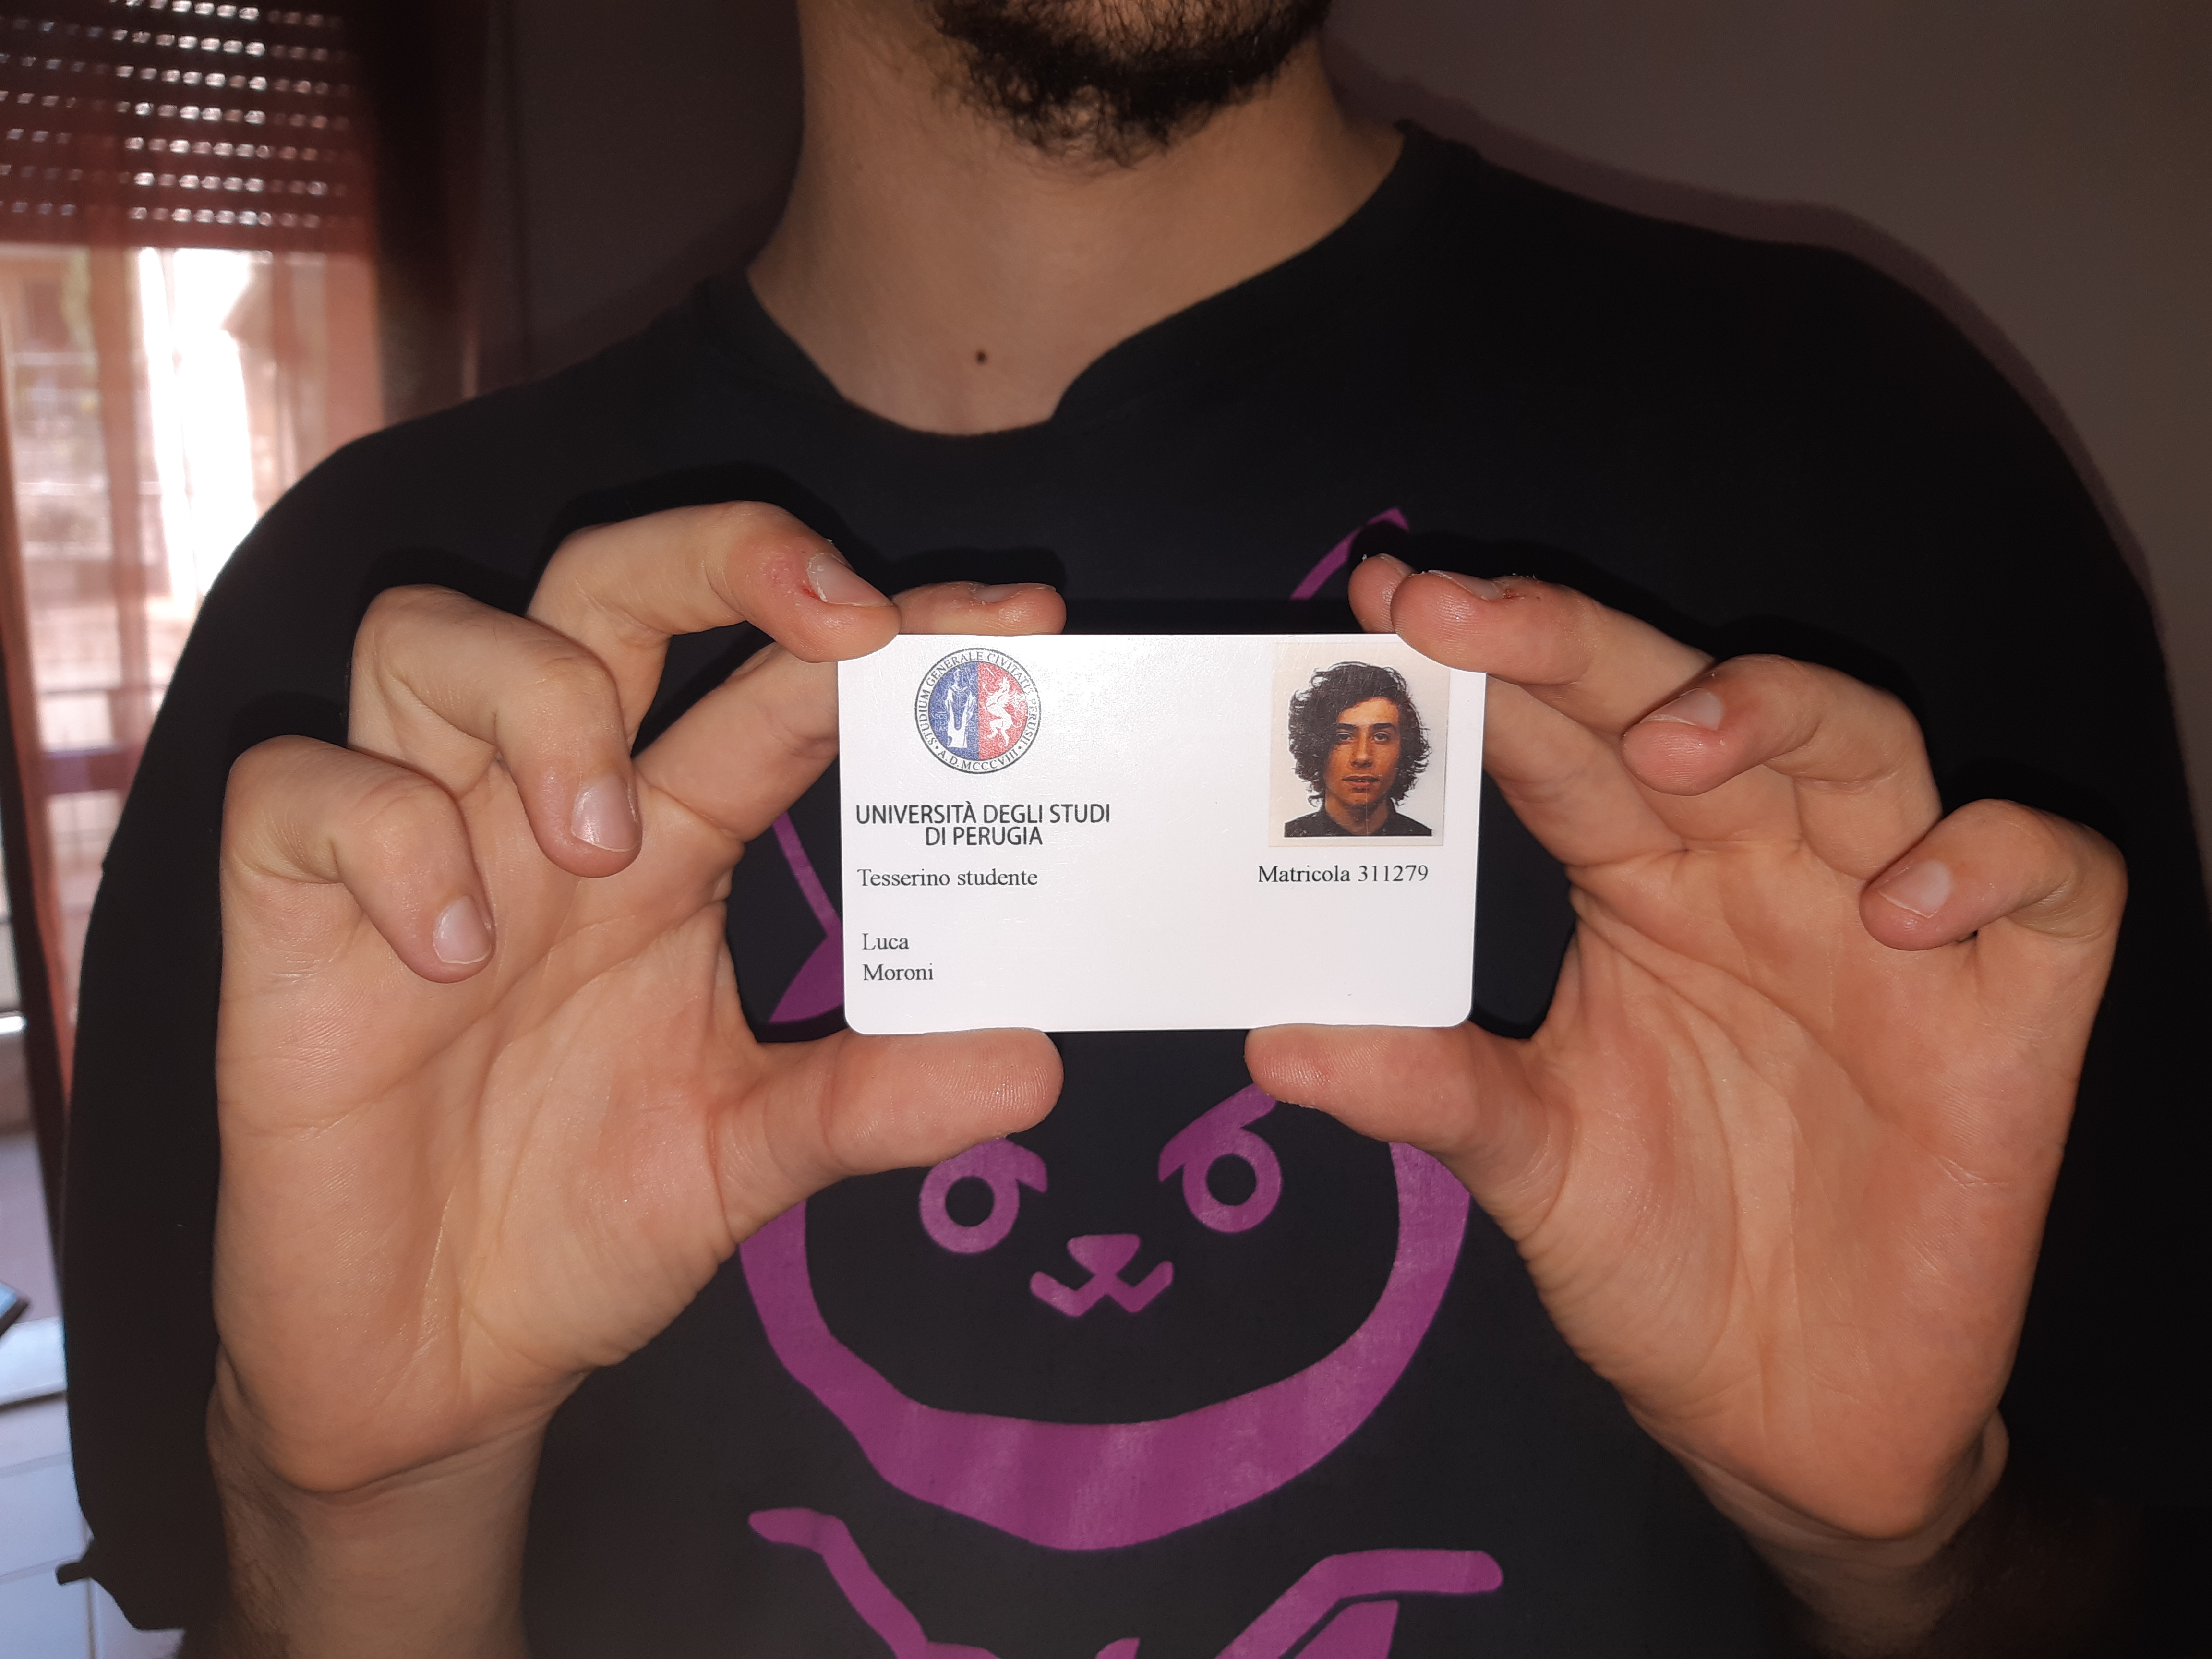
\includegraphics[width=.7\linewidth]{test_tesserino.jpg}
     \caption{Caso di Test TESSERINO}\label{Fig:}
   \end{minipage}\hfill
   \begin{minipage}{0.48\textwidth}
     \centering
     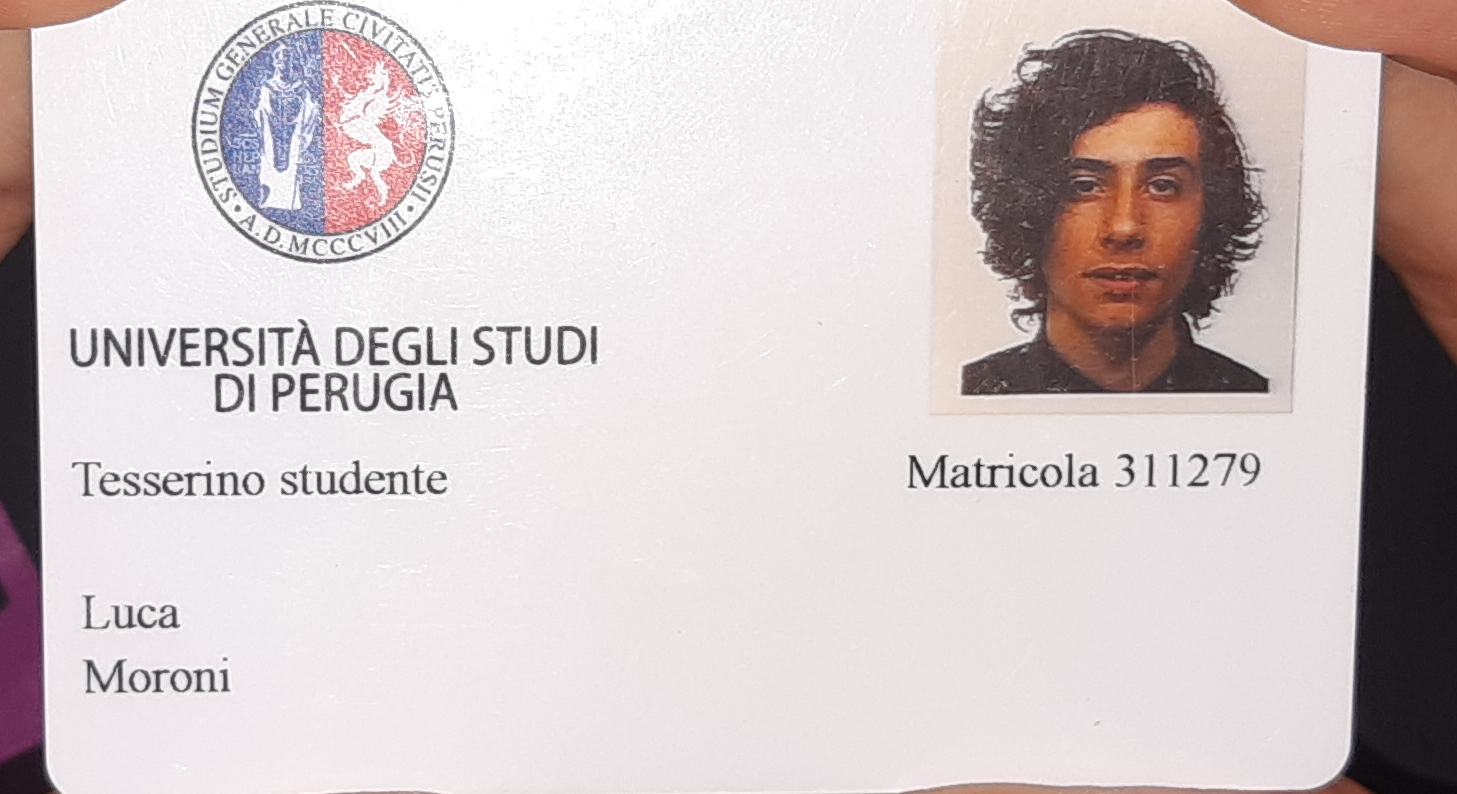
\includegraphics[width=.7\linewidth]{test_tesserino_cutting.jpg}
     \caption{Document Cutted}\label{Fig:}
   \end{minipage}
\end{figure}

Output:
\inputminted{python}{test_tesserino.py}

\begin{figure}[!htb]
   \begin{minipage}{0.48\textwidth}
     \centering
     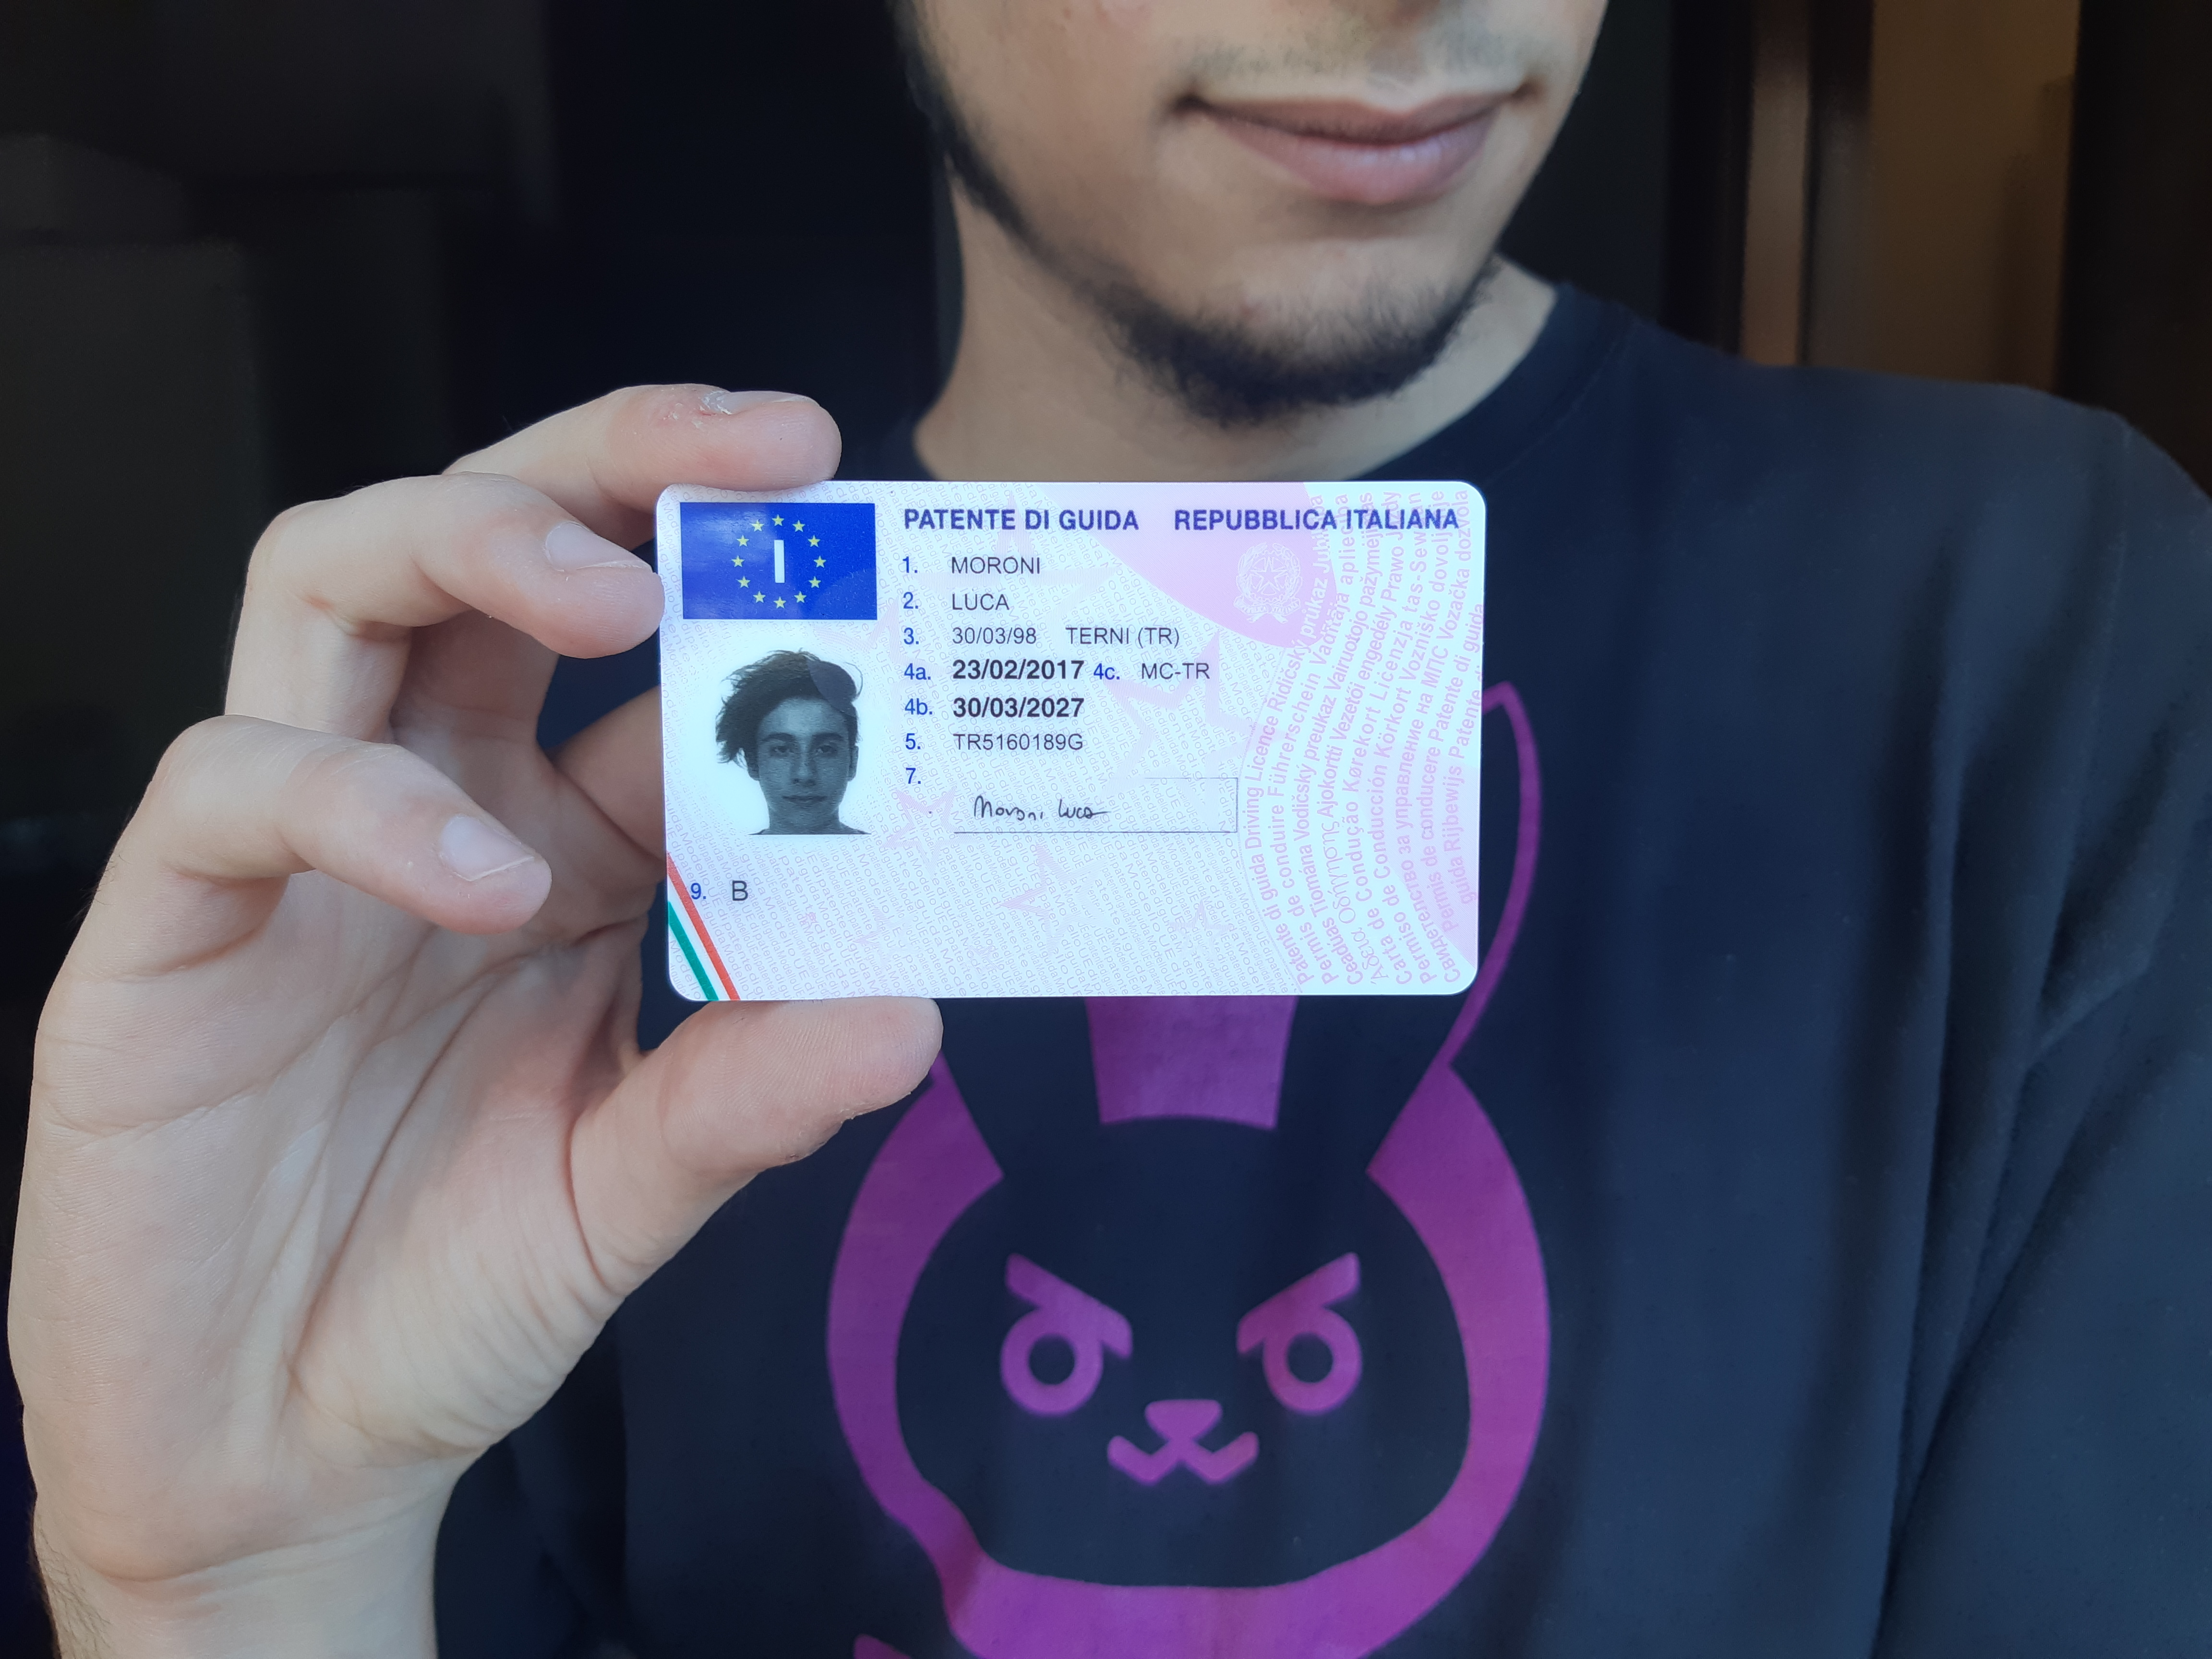
\includegraphics[width=.7\linewidth]{test_patente.jpg}
     \caption{Caso di Test PATENTE}\label{Fig:}
   \end{minipage}\hfill
   \begin{minipage}{0.48\textwidth}
     \centering
     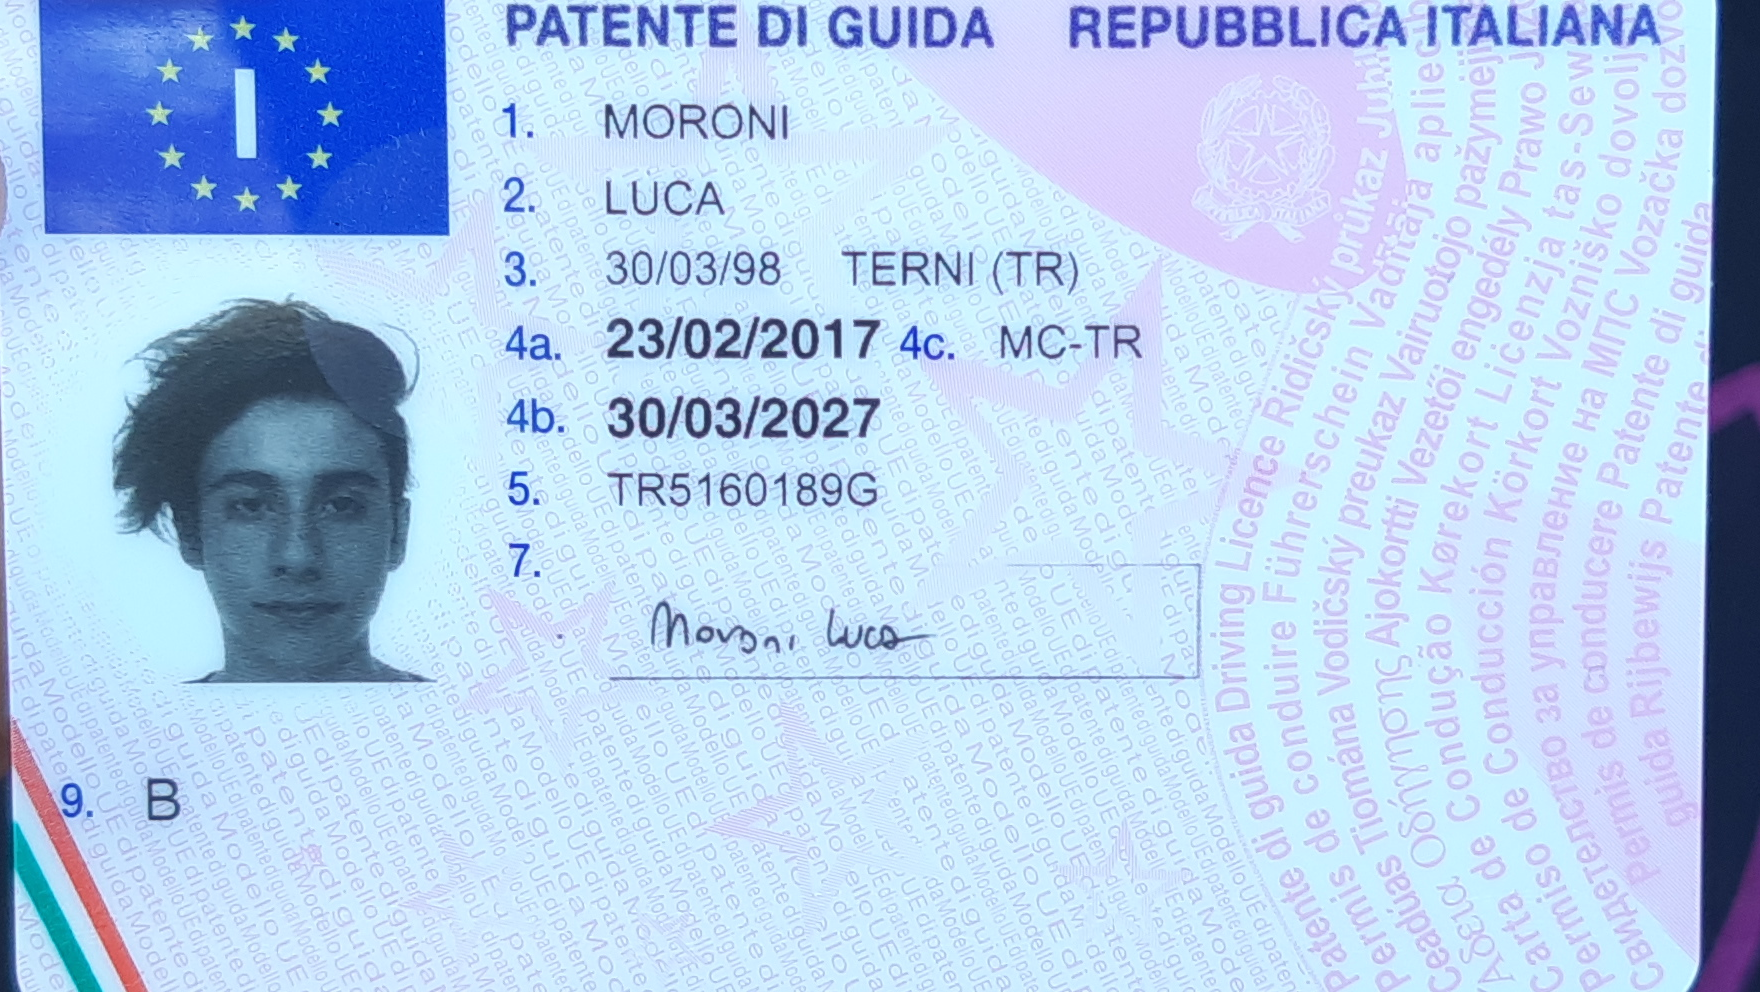
\includegraphics[width=.7\linewidth]{test_patente_cutting.jpg}
     \caption{Document Cutted}\label{Fig:}
   \end{minipage}
\end{figure}

Output:
\inputminted{python}{test_patente.py}

\begin{figure}[H]
    \caption{Caso di test BG}
    \centering
    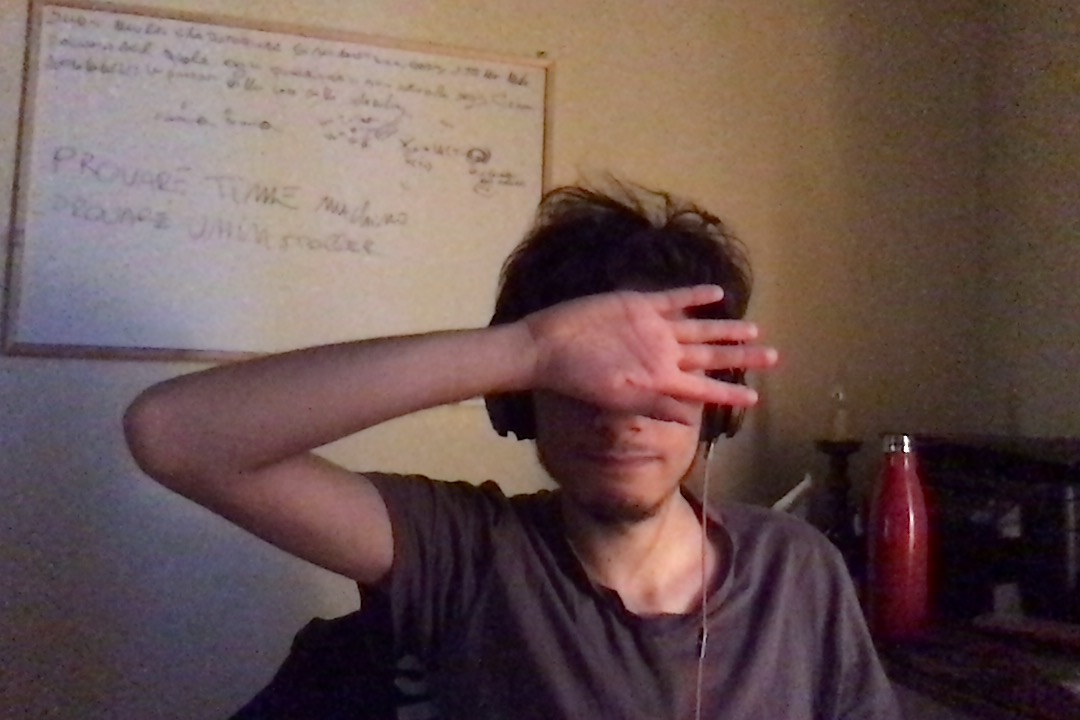
\includegraphics[width=\textwidth,height=\textheight,keepaspectratio]{test_background.jpg}
\end{figure}

Output:
\inputminted{python}{test_background.py}

\pagebreak

\section{Notebook Jupyter}
\label{s:notebook}

\setminted[python]{
    linenos,
    breaklines,
    breakbefore=/,
    breakafter=(,
    frame=single,
    framesep=2mm
}
\setminted[text]{
    breaklines,
    breakbefore=/,
    breakafter=(,
    frame=single,
    framesep=2mm
}

Segue una copia commentata di un notebook Jupyter che è stato utilizzato
per eseguire il training del dataset di esempio in Google Colab. Per
l'ultima versione dell'originale consultare la repo git.

\subsection{Preparazione dei prerequisiti}

Configuriamo la versione per le librerie utilizzate che ne richiedono
una in particolare.

\begin{minted}{python}
print("DOCUMENT RECOGNITION Training")
%tensorflow_version 1.x
!pip install keras==2.0.8
\end{minted}

Cloniamo la repo git di \mrcnn\ e la installiamo, dopodiché proseguiamo
il lavoro nella directory della repo stessa.

\begin{minted}{python}
# setup the library and its dependencies
!git clone https://github.com/matterport/Mask_RCNN.git
%cd Mask_RCNN
!python setup.py install
!pip install -r requirements.txt
\end{minted}

Montiamo la cartella Google Drive nella quale il dataset è stato
preventivamente caricato.

\begin{minted}{python}
from google.colab import drive
drive.mount('/content/drive')
\end{minted}

Scarichiamo un file di pesi preallenato su Microsoft COCO, un dataset
pensato per il riconoscimento di oggetti in contesti non isolati sul
quale faremo transfer learning per le nostre classi di documenti.

\begin{minted}{python}
!wget https://github.com/matterport/Mask_RCNN/releases/download/v2.0/mask_rcnn_coco.h5
\end{minted}

\subsection{Inizializzazione}

Importiamo le librerie e prepariamo i percorsi.

\begin{minted}{python}
import os
import sys
import json
import datetime
import numpy as np
import skimage.draw
import cv2
from mrcnn.visualize import display_instances
import matplotlib.pyplot as plt

# Root directory of the project
ROOT_DIR = os.path.abspath("./")

# Import Mask RCNN
sys.path.append(ROOT_DIR)
from mrcnn.config import Config
from mrcnn import model as modellib, utils

# Path to trained weights file
COCO_WEIGHTS_PATH = os.path.join(
    ROOT_DIR, "mask_rcnn_coco.h5")
\end{minted}

Definiamo la nostra configurazione di \mrcnn\ derivando la classe
\texttt{Config}.

\begin{minted}{python}
class CustomConfig(Config):
    """
    Configuration for training on the dataset provided on
    Google Drive. Derives from the base Config class and
    overrides some values.
    """
    # Give the configuration a recognizable name
    NAME = "document"

    # We use a GPU with 12GB memory, which can fit two
    # images. Adjust down if you use a smaller GPU.
    IMAGES_PER_GPU = 2

    # Number of classes (including background)
    NUM_CLASSES = 1 + 2  # Background + documents

    # Number of training steps per epoch
    STEPS_PER_EPOCH = 150

    VALIDATION_STEPS = 25

    LEARNING_RATE=0.006

    # Skip detections with < 90% confidence
    DETECTION_MIN_CONFIDENCE = 0.9
\end{minted}

CustomDataset estende la classe Dataset di \mrcnn\ per
permettere il caricamento dei dati dal particolare albero di
cartelle in cui abbiamo memorizzato il dataset.
Per ``mask'' (maschera) si intende la regione di ogni
immagine occupata dall'oggetto da riconoscere.

\begin{minted}{python}
class CustomDataset(utils.Dataset):
    def load_custom(self, dataset_dir, training=True):
        """
        Loads dataset from our directory structure. Every
        image containing directory must have inside an
        annotations file named "via_regions.json"

        Parameters:
        dataset_dir: path of the root folder of the dataset
        training: switch between training and validating
                  datasets
        """

        if training:
            dataset_dir = os.path.join(dataset_dir, "training/")
        else:
            dataset_dir = os.path.join(dataset_dir, "validating/")

        # Add classes.
        self.add_class("dataset", 1, "tesserino")
        self.add_class("dataset", 2, "patente")

        # Load annotations
        # VGG Image Annotator saves each image in the form:
        # { 'filename': '28503151_5b5b7ec140_b.jpg',
        #   'regions': {
        #       '0': {
        #           'region_attributes': {},
        #           'shape_attributes': {
        #               'all_points_x': [...],
        #               'all_points_y': [...],
        #               'name': 'polygon'}},
        #       ... more regions ...
        #   },
        #   'size': 100202
        # }
        # We mostly care about the x and y coordinates of
        # each region

        dir_list = [
            dir_
            for dir_ in os.listdir(dataset_dir)
            if os.path.isdir(os.path.join(dataset_dir, dir_))
        ]

        for dir_ in dir_list:
            iter_dir = os.path.join(dataset_dir, dir_ + "/")

            print("iterating: {0} ...".format(iter_dir))

            annotations1 = json.load(open(
                os.path.join(iter_dir, "via_regions.json")))
            # don't need the dict keys:
            annotations = list(annotations1.values())

            # The VIA tool saves images in the JSON even if
            # they don't have any annotations. Skip
            # unannotated images.
            annotations = [
                a for a in annotations if a['regions']]

            # Add images
            for a in annotations:
                # Get the x, y coordinaets of points of the
                # polygons that make up the outline of each
                # object instance. There are stores in the
                # shape_attributes (see json format above)
                polygons = [
                    (
                        r['region_attributes'],
                        r['shape_attributes']
                    )
                    for r in a['regions']
                ]

                # load_mask() needs the image size to convert
                # polygons to masks. Unfortunately, VIA
                # doesn't include it in JSON, so we must read
                # the image. This is only managable since the
                # dataset is tiny.
                image_path = os.path.join(
                    iter_dir, a['filename'])
                image = skimage.io.imread(image_path)
                height, width = image.shape[:2]

                self.add_image(
                    "dataset",
                    image_id=a['filename'],
                    path=image_path,
                    width=width, height=height,
                    polygons=polygons)

    # this method is invoked iteratively from the net during
    # training (GRADIENT DESCEND)
    def load_mask(self, image_id):
        """
        Generate instance masks for an image.

        Returns:
        masks: A bool array of shape [height, width,
               instance_count] with one mask per instance.
        class_ids: a 1D array of class IDs of the instance
                   masks.
        """

        # If not a dataset image, delegate to parent class.
        image_info = self.image_info[image_id]
        if image_info["source"] != "dataset":
            return super().load_mask(image_id)

        # Convert polygons to a bitmap mask of shape
        # [height, width, instance_count]
        info = self.image_info[image_id]
        mask = np.zeros(
            [
                info["height"],
                info["width"],
                len(info["polygons"])
            ],
            dtype=np.uint8)

        class_ids = list()
        for i, p in enumerate(info["polygons"]):
            # Get indices of pixels inside the polygon and
            # set them to 1
            rr, cc = skimage.draw.polygon(
                p[1]['all_points_y'], p[1]['all_points_x'])
            mask[rr, cc, i] = 1
            class_ids.append(
                self.class_names.index(p[0]['name']))

        # Return mask, and array of class IDs of each
        # instance. Since we have one class ID only, we
        # return an array of 1s
        return (
            mask.astype(np.bool),
            np.asarray(class_ids, dtype='int32'))

    def image_reference(self, image_id):
        """
        Return the path of the image.
        """
        info = self.image_info[image_id]
        print("reference...")
        if info["source"] == "dataset":
            print(info["path"])
            return info["path"]
        else:
            super().image_reference(image_id)
\end{minted}

Funzione di training.
Si occupa delle operazioni di carimento dei dataset di
training e validating ed esegue il trainig effuttuando tuning
di alcuni parametri.

\begin{minted}{python}
classes_ = None

def train(model):
    """Train the model."""

    global classes_

    # Training dataset.
    dataset_train = CustomDataset()
    dataset_train.load_custom(
        "/content/drive/My Drive"
        + "/Ing_sw_testing/document_dataset/",
        training=True)
    dataset_train.prepare()

    classes_ = dataset_train.class_names

    # Validation dataset
    dataset_val = CustomDataset()
    dataset_val.load_custom(
        "/content/drive/My Drive"
        + "/Ing_sw_testing/document_dataset/",
        training=False)
    dataset_val.prepare()

    # *** This training schedule is an example. ***
    # ***         Update to your needs          ***
    # Since we're using a very small dataset, and starting
    # from COCO trained weights, we don't need to train too
    # long. Also, no need to train all layers, just the
    # heads should do it.
    print("Training network heads")
    model.train(
        dataset_train,
        dataset_val,
        learning_rate=config.LEARNING_RATE,
        epochs=10,
        layers='heads')
\end{minted}

Istanziamo un oggetto di configurazione \texttt{CustomConfig}.

\begin{minted}{python}
config = CustomConfig()
config.display()
\end{minted}

Creiamo un modello in modalità training e carica i pesi MSCOCO per
effettuare il transfer learning.

\begin{minted}{python}
model = modellib.MaskRCNN(
    mode="training", config=config, model_dir="./")

weights_path = COCO_WEIGHTS_PATH

model.load_weights(
    weights_path,
    by_name=True,
    exclude=[
        "mrcnn_class_logits", "mrcnn_bbox_fc",
        "mrcnn_bbox", "mrcnn_mask"])

train(model)
\end{minted}

Salviamo i nuovi pesi ottenuti tramite transfer learning.

\begin{minted}{python}
import time
model_path = 'mask_rcnn_' + '.' + str(time.time()) + '.h5'
model.keras_model.save_weights(model_path)
print(model_path)
\end{minted}

Scarichiamo i pesi.

\begin{minted}{python}
from google.colab import files
files.download(model_path)
\end{minted}

Definiamo una nuova classe derivata da \texttt{InferenceConfig}, usata
per effettuare un piccolo test finale sulla nostra rete.

\begin{minted}{python}
class InferenceConfig(CustomConfig):
    # Set batch size to 1 since we'll be running inference on
    # one image at a time.
    # Batch size = GPU_COUNT * IMAGES_PER_GPU
    GPU_COUNT = 1
    IMAGES_PER_GPU = 1
    DETECTION_MIN_CONFIDENCE = 0.9

config = InferenceConfig()
config.display()
\end{minted}

Creiamo un modello \mrcnn\ in modalità inferenza caricando i nuovi pesi
da testare.

\begin{minted}{python}
model = modellib.MaskRCNN(
    mode="inference", config=config,  model_dir="./")

model.load_weights(model_path, by_name=True)
\end{minted}

Eseguiamo la \texttt{detection} su un'immagine non utilizzata per
allenare il modello.

\begin{minted}{python}
# Run object detection
image = skimage.io.imread(
    "/content/drive/My Drive/Ing_sw_testing"
    + "/document_dataset/testing/test2.jpg")
results = model.detect([image], verbose=1)

# Display results
r = results[0]

print(classes_)

display_instances(
    image, r['rois'], r['masks'],
    r['class_ids'], classes_, r['scores'])

print(r['rois'])
\end{minted}

\pagebreak

\textbf{Output}:

\begin{minted}{text}
Processing 1 images
image         shape: (426, 640, 3)      min:    0.00000 max:  255.00000 uint8
molded_images shape: (1, 1024, 1024, 3) min: -123.70000 max:  138.20000 float64
image_metas   shape: (1, 15)            min:    0.00000 max: 1024.00000 float64
anchors       shape: (1, 261888, 4)     min:   -0.35390 max:    1.29134 float32
['BG', 'tesserino', 'patente']
\end{minted}

\begin{figure}[H]
    \caption{Esito del Test}
    \centering
    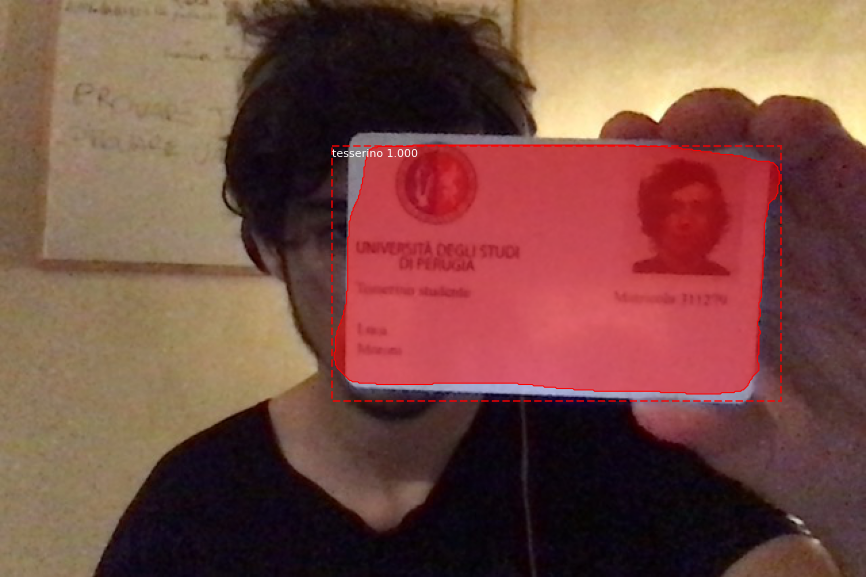
\includegraphics[width=\textwidth,height=\textheight,keepaspectratio]{document_recognition_29_1.png}
\end{figure}

\begin{minted}{text}
[[107 245 296 577]]
\end{minted}

\end{document}
